\documentclass[12pt,a4paper]{article}
\usepackage[utf8]{inputenc}
\usepackage[english]{babel}
\usepackage{enumerate}
\usepackage{amsmath}
\usepackage{amsfonts}
\usepackage{amssymb}
\usepackage{graphicx}
\usepackage{fourier}
\usepackage[left=2cm,right=2cm,top=2cm,bottom=2cm]{geometry}
\usepackage{commath}
\usepackage{cancel}
\usepackage{placeins}
\author{Juan Carlos Apitz, ID 012523821}
\title{STAT572 - In Class Test 1}
\begin{document}

\maketitle

\section*{Question 1}

\textit{Part a.}

\textbf{Procedure}
For this question we first define a function handle $f(x)$ to calculate the Slash distribution per the question. Then:

\begin{enumerate}
\item{
Generate a set of uniform random values between 0 and 1, call it $u$.
}

\item{
Generate values which are necessarily between 0 and 1 from the Slash CDF, call it $F(x)$.
}

\item{
If $F(x)>u$, then we deem this $x$ value as having come from the Slash distribution and we keep it in the random sample, otherwise we discard the particular $x$ value. We do this for all values of $x$ in the domain, which for the Slash is infinite, so we choose the domain $(-5<x<5)$ which contains most of the density of the Slash distribution. This is our random sample.
}
\end{enumerate}

\textbf{Code}\\
\textit{Slash PDF}
\begin{verbatim}
function [x] = slash(y)
x = zeros(size(y));
for i = 1:length(y)
    if y(i) ~= 0
        x(i) = (1-exp(-y(i).^2/2))/((y(i).^2)*sqrt(2*pi));
    else
        x = 1/(2*sqrt(2*pi));
    end
end
\end{verbatim}

\textit{Script to Generate Data and Analysis}

\begin{verbatim}
%initialize parameters
n = 100; % sample size
M = 1000;
x=linspace(-5,5,100);
F=zeros(size(x));
rs=zeros(size(x));
u=rand(1,200);
% Monte Carlo loop
par = zeros(1,M);

% Loop thru uniforms and x vector picking x's that meet criteria
for i=1:length(u)
    for j=1:length(x)
        if quadgk(@(x)slash(x),-inf,x(j))<u(i)
            F(j)=1;
        else
            F(j)=quadgk(@(x)slash(x),-inf,x(j));
        end
    end
    if min(F) ~= 1
        l=find(F==min(F));
        rs(i)=x(l);
    end
end

% plots
figure(1)
HIST =  hist(rs);
bar(-5:1.1:5,HIST/length(u),1,'w')
title('Frequecy Histogram of Slash Random Sample')
hold on
plot(x,g);
axis([-6 6 0 0.25])
hold off

figure(2)
plot(x,y);

figure(3)
cdfplot(rs);

% Monte Carlo
M= 1000;
MUHAT= mean(rs);
SIGMAHAT= std(rs);

for i= 1:M
rsho = normrnd(1,SIGMAHAT);
trs(i)= mean(rsho);
end

alpha= 0.05;
ind= find( trs >= median(rs));
PVAL= length(ind)/M;
\end{verbatim}

\textbf{Results}

\begin{figure}[ht!]
\begin{center}
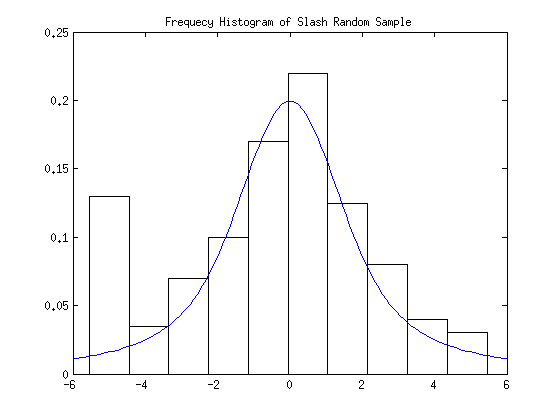
\includegraphics[scale=.9]{q1_density.png}
\caption{Density Histogram of Slash Random Sample}
\label{q1 fig1}
\end{center}
\end{figure}
\FloatBarrier

\begin{figure}[ht!]
\begin{center}
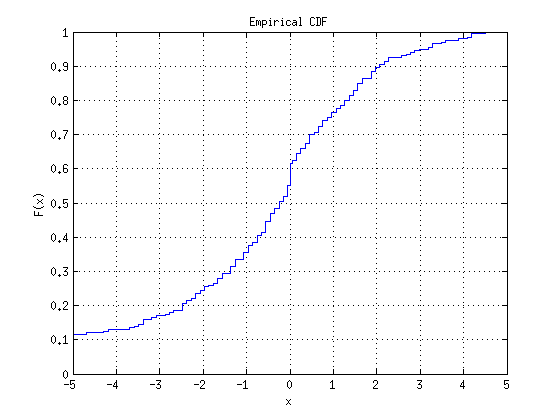
\includegraphics[scale=.9]{q1_empirical.png}
\caption{Empirical CDF Slash Random Sample}
\label{q1 fig2}
\end{center}
\end{figure}
\FloatBarrier

\begin{figure}[ht!]
\begin{center}
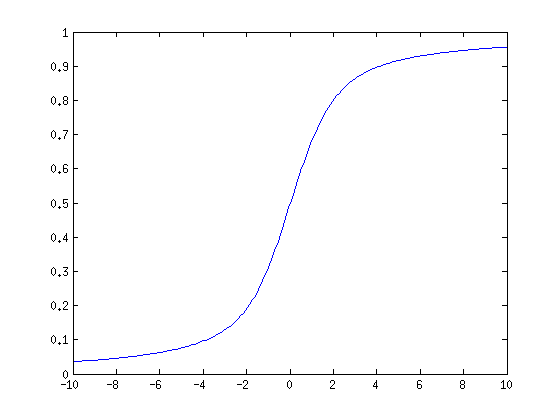
\includegraphics[scale=.9]{q1_theoretical.png}
\caption{Theoretical CDF of Slash Dist}
\label{q1 fig1}
\end{center}
\end{figure}
\FloatBarrier

As expected the, theoretical Slash CDF generated from the pdf function per the question closely resembles the cdf generated by the random sample.

\textit{Part b.}

\textbf{Procedure}
To generate a Monte Carlo simulation  to perform hypothesis testing on the population median, i.e.

\[H_o: m\leq 1\text{ vs. }H_1 > 1\]

\begin{enumerate}
\item{
Doing hypothesis testing about the median for the Slash distribution is similar to doing hypothesis testing for the mean because the Slash distribution is symmetric, just like the normal except that it has fatter tails.\\

We calculate the test statistic of from the random sample generated by the Slash of size $200$. In this case we calculate the median $m$ from the random sample generated in a).
}

\item{
Then we use the normal as a pseudo population, which is reasonable since the normal and the Slash share many characteristics. We sample from the normal under the null hypothesis, i.e. the pseudo population is $N\bigr(1,\sigma^2_{slash}\bigr)$. I set up the simulation at $M=1000$.
}

\item{
For each sample we calculate the median $m_o$, and after the Monte Carlo sampling is complete we have a vector of 1000 $m_o$, medians with an expected value of 1.
}

\item{
Then we estimate the p-value by looking at the sample of medians with expected value 1 generated by the Monte Carlo process and seeing what percent of these values are above the median of the random sample generated in a). That is we count how many of the 1000 medians generated from the simulation are greater than the median of the random sample generated in a) divide by 1000, the number of Monte Carlo simulation. We obtain a value of $65.6\%$. 
}

\item{
From the above result we conclude that the random sample does not come from a distribution that is normal with median/mean that is $>1$, we fail to reject the null hypothesis that $m\leq1$.
}


\end{enumerate}

\textbf{Code}\\
\begin{verbatim}
% Monte Carlo
M= 1000;
MUHAT= mean(rs);
SIGMAHAT= std(rs);

for i= 1:M
rsho = normrnd(1,SIGMAHAT);
trs(i)= median(rsho);
end

ind= find( trs >= median(rs));
PVAL= length(ind)/M;
\end{verbatim}

\textbf{Results}\

\begin{verbatim}

>> test

PVAL =

    0.656
\end{verbatim}
\end{document}
